\chapter{Monad Transformers}

Monad transformers offer an additional benefit to monadic programming: by providing a
library of different monads and types and functions for combining these monads, it is possible
to create custom monads simply by composing the necessary monad transformers. [Monad Transformers Step by Step]\\

In real world application, it is often the case that a combination different type of action is required to put into one function.Monad transformer provide a new way to glue them together.

\section{State Transformer}
A value of type \textbf{(ST a s)} is a computation which transforms a state index by type s ,and delivers a value of type a ,You can think of it as a box ,like this 
\begin{figure}[H]
  \centering
	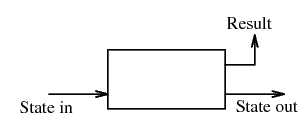
\includegraphics[width=0.60\textwidth]{pic/c3/state.png}
	\caption{Diagram illustrating a state monad}
\end{figure}
[lazy functional state thread]
\\

First , a state transformer is a monad, other than encapsulating a data behind signature , it encapsulated a computation,the \textbf{runState} function provide by the state monad is an escape function that allow us to extract is state logic from the computation,by feeding the state computation function with an initial state,we are able to get the final state.Other type of escape function is provided to extract computation as well.

Second,a state transformer can accept other monads to combine the computation which state as well as other logic says the IO logic.


\section{Error Transformer}
ErrorT monad transformer can be used to add error handling to another monad. Below is an example how to combine it with an IO monad:

\begin{hcode}
main = do
  -- runErrorT removes the ErrorT wrapper
  r <- runErrorT calculateLength
  reportResult r

-- Asks user for a non-empty string and returns its length.
-- Throws an error if user enters an empty string.
calculateLength :: LengthMonad Int
calculateLength = do
  -- all the IO operations have to be lifted to the IO monad in the monad stack
  liftIO $ putStrLn "Please enter a non-empty string: "
  s <- liftIO getLine
  if null s
    then throwError "The string was empty!"
    else return $ length s
\end{hcode}



\section{Putting All Together}